%=======================================================================
\section{Proposed Solution}
\label{sec:solution}
%=======================================================================

Problem $\mathscr{P}_{2}$ is a robust assignment problem whose only coupling across UEs is the capacity of the
serving nodes. SENTINEL solves it in three steps. The minimax over scenarios is handled by a classical outer loop on
scenario weights, so that every subproblem handed to a quantum sampler has a linear objective. Each domain's
subproblem is encoded as a compact QUBO over its decision variables and a few capacity-slack bits, with the one-hot
constraint enforced by the mixer of the quantum circuit rather than by a penalty. The domains are coordinated through
the sharing form of ADMM. Every schedule produced at any point of the procedure is certified exactly by its worst-case
AoII over $\mathscr{L}$, so the procedure can be stopped at any time with a valid guarantee in hand.

%-----------------------------------------------------------------------
\subsection{Scenario-Weight Dualization of the Minimax}
\label{sec:dual}
%-----------------------------------------------------------------------

Write $c^{(\ell)}(\mathbf{x})=\frac{1}{|\mathscr{U}|}\sum_{i}\sum_{(m,q,h)\in\mathscr{A}_i}\psi^{(\ell)}_{imqh}x_{imqh}$
for the network AoII under scenario $\ell$. For any $\mathbf{x}$ and any weight vector $\mathbf{w}$ in the simplex
$\Delta_L=\{\mathbf{w}\geq 0,\ \sum_\ell w_\ell=1\}$,
\begin{equation}
    \max_{\ell\in\mathscr{L}} c^{(\ell)}(\mathbf{x})
    =\max_{\mathbf{w}\in\Delta_L}\sum_{\ell\in\mathscr{L}} w_\ell\, c^{(\ell)}(\mathbf{x}),
    \label{eq:dual_max}
\end{equation}
so $\mathscr{P}_{2}$ is $\min_{\mathbf{x}}\max_{\mathbf{w}\in\Delta_L}\mathbf{w}^{\top}\mathbf{c}(\mathbf{x})$. We
approach the saddle point by alternating an inner step on $\mathbf{x}$ for fixed $\mathbf{w}$, which is the step
handed to the quantum sampler, with an exponentiated-gradient step on $\mathbf{w}$~\cite{Arora2012}:
\begin{align}
    \mathbf{x}^{(t)} &\in \arg\min_{\mathbf{x}\ \text{s.t. D1--D4}}\ \sum_{\ell} w^{(t)}_\ell\, c^{(\ell)}(\mathbf{x}),
    \label{eq:inner}\\
    \eta^{(t)} &= \max_{\ell} c^{(\ell)}(\mathbf{x}^{(t)}),
    \label{eq:cert}\\
    w^{(t+1)}_\ell &\propto w^{(t)}_\ell \exp\!\bigl(\sigma\, c^{(\ell)}(\mathbf{x}^{(t)})/\eta^{(t)}\bigr),
    \label{eq:eg}
\end{align}
with step $\sigma>0$ and $\mathbf{w}^{(1)}$ uniform, for $T$ outer iterations. The weights move toward the scenarios
that hurt the current schedule most, and the next inner solve is pulled toward schedules that do better on them.
Equation~\eqref{eq:cert} is the exact worst-case AoII of $\mathbf{x}^{(t)}$ over $\mathscr{L}$, computed in
$\mathcal{O}(L|\mathscr{U}|)$; SENTINEL returns the iterate with the smallest $\eta^{(t)}$ together with that value as
its certificate. Because the inner problem~\eqref{eq:inner} has a linear objective, it needs neither the epigraph
variable nor the scenario slacks of a direct minimax encoding. In our instances those auxiliary registers,
$M_\eta+\sum_\ell W_\ell$ qubits per domain, outnumbered the decision qubits.

%-----------------------------------------------------------------------
\subsection{Candidate Pruning}
\label{sec:pruning}
%-----------------------------------------------------------------------

The pre-elimination of Section~IV-A removes inadmissible combinations. We further retain, for each UE, only the
$\kappa$ admissible combinations with the smallest worst-case cost $\max_\ell\psi^{(\ell)}_{imqh}$, plus the best
combination at every other visible node so that the capacity coupling is preserved, and denote the result
$\mathscr{C}_i\subseteq\mathscr{A}_i$. The number of decision qubits per UE is then at most $\kappa+|\mathscr{M}|$
instead of $\sum_m Q_mH_i$. Pruning could in principle discard an optimal combination that is individually poor but
relieves a congested node; with $\kappa=4$ this did not happen on any of the instances of Section~VI, where the
exact optimum over $\mathscr{C}$ equalled the exact optimum over $\mathscr{A}$ from 10 to 100 UEs.

%-----------------------------------------------------------------------
\subsection{Compact Domain QUBO}
\label{sec:compact_qubo}
%-----------------------------------------------------------------------

For domain $k$ with weights $\mathbf{w}$ and ADMM state $(\mathbf{z}_k,\mathbf{u}_k)$, let
$a_v=\frac{1}{|\mathscr{U}|}\sum_\ell w_\ell\psi^{(\ell)}_v$ for $v=(i,m,q,h)$, $i\in\mathscr{U}_k$,
$(m,q,h)\in\mathscr{C}_i$, and let $b_m(\mathbf{x}_k)=\sum_{i\in\mathscr{U}_k}\sum_{(m,q,h)\in\mathscr{C}_i}
\bar\beta^q_m x_{imqh}$ be the bandwidth that domain $k$ uses at node $m$. Satellites visible only to domain $k$ form
$\mathscr{S}^{\mathrm{o}}_k$; those shared with other domains form $\mathscr{S}^{\mathrm{sh}}_k$. The binary vector
$\mathbf{y}_k=(\mathbf{x}_k,\boldsymbol{\nu}_k)$ holds the decision variables and, for each node
$m\in\mathscr{S}^{\mathrm{o}}_k\cup\mathscr{B}_k$, a capacity slack $\nu_m=\Delta_\beta\sum_{b}2^b y_{m,b}$ of
$W_m=\lceil\log_2(B_m/\Delta_\beta+1)\rceil$ bits, where the bandwidth levels and capacities are integer multiples of
$\Delta_\beta$. The domain QUBO is
\begin{align}
    F_k(\mathbf{y}_k)=\sum_{v}a_v x_v
    &+\lambda\!\!\sum_{m\in\mathscr{S}^{\mathrm{o}}_k\cup\mathscr{B}_k}\!\!\bigl(b_m(\mathbf{x}_k)+\nu_m-B_m\bigr)^2
    \nonumber\\
    &+\frac{\varrho}{2}\sum_{j\in\mathscr{S}^{\mathrm{sh}}_k}\bigl(b_j(\mathbf{x}_k)-z_{jk}+u_{jk}\bigr)^2 .
    \label{eq:Fk_compact}
\end{align}
The first term is the weighted AoII cost, the second enforces the capacity of the nodes that belong to the domain
alone, and the third is the augmented-Lagrangian coordination term for the shared satellites, with penalty parameter
$\varrho$. Constraint D1 does not appear: the mixer of Section~V-D keeps every UE group one-hot, so on the subspace
the circuit can reach, $x_vx_{v'}=0$ for two candidates of the same UE and the corresponding entries of the QUBO
matrix are dropped. The matrix $\mathbf{Q}^{(k)}$ collects the linear coefficients of $F_k$ on its diagonal, since
$y^2=y$ for binary $y$, and the pairwise coefficients split between the two symmetric off-diagonal entries.

\begin{proposition}
\label{prop:penalty}
Let $\bar a_k=\sum_{i\in\mathscr{U}_k}\max_{v\in\mathscr{C}_i}a_v$ and let $\Gamma_k^{\max}$ and $\Gamma_k^{\min}$ be
the largest and smallest values of the coordination term over one-hot assignments of domain $k$. If
\begin{equation}
    \lambda>\frac{\bar a_k+\Gamma_k^{\max}-\Gamma_k^{\min}}{\Delta_\beta^{2}}
    \label{eq:lambda_sufficient}
\end{equation}
and the domain problem is feasible, then every one-hot minimizer of $F_k$ satisfies the capacity constraints of
$\mathscr{S}^{\mathrm{o}}_k\cup\mathscr{B}_k$ and minimizes the weighted cost plus coordination term over the
feasible one-hot assignments.
\end{proposition}

\begin{proof}
Over one-hot assignments the cost term lies in $[0,\bar a_k]$. For a feasible assignment whose slack bits represent
the unused capacity exactly, the penalty vanishes and $F_k\leq\bar a_k+\Gamma_k^{\max}$. For an assignment that
exceeds the capacity of some node, the residual of that node is a positive integer multiple of $\Delta_\beta$ for
every choice of slack bits, since the slack is non-negative, so the penalty is at least $\lambda\Delta_\beta^2$ and
$F_k\geq\lambda\Delta_\beta^2+\Gamma_k^{\min}>\bar a_k+\Gamma_k^{\max}$. No infeasible one-hot assignment is
therefore a minimizer, and on the feasible set $F_k$ equals the cost plus coordination term once the slack bits are
chosen to cancel the penalty.
\end{proof}

The bound is taken over one-hot assignments because that is the subspace the circuit explores. Taking it over the
whole hypercube, as a penalty analysis of a transverse-field QAOA would require, inflates $\lambda$ by more than an
order of magnitude and flattens the energy landscape to the point where neither simulated annealing nor QAOA finds
a feasible point; this was the behaviour of the epigraph encoding and is quantified in Section~VI-D. The number of
qubits of domain $k$ is
\begin{equation}
    \hat{N}_k=\sum_{i\in\mathscr{U}_k}|\mathscr{C}_i|+\sum_{m\in\mathscr{S}^{\mathrm{o}}_k\cup\mathscr{B}_k}W_m,
    \label{eq:Nk_compact}
\end{equation}
independent of $L$. With the parameters of Section~VI and two domains, this is 22, 34, 46 and 58 qubits per domain at
5, 10, 15 and 20 UEs, against 120 to 260 for the epigraph encoding of the same instances
(Fig.~\ref{fig:qubits}).

\begin{figure}[!t]
\centering
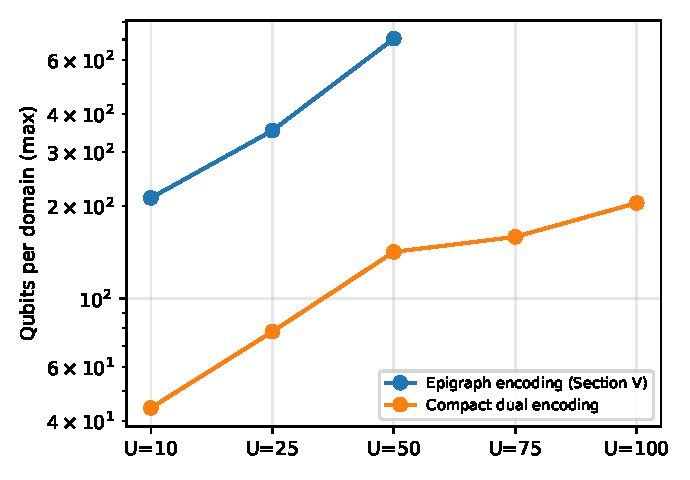
\includegraphics[width=0.85\columnwidth]{figures/qubits_compact_vs_epigraph.pdf}
\caption{Qubits per domain of the compact formulation~\eqref{eq:Nk_compact} and of the direct epigraph encoding of
$\mathscr{P}_3$ (one epigraph register and one slack register per scenario) for the instances of Section~VI.}
\label{fig:qubits}
\end{figure}

%-----------------------------------------------------------------------
\subsection{Ising Mapping and XY-Mixer QAOA}
\label{sec:qaoa}
%-----------------------------------------------------------------------

The QUBO is mapped to an Ising Hamiltonian through the substitution $y_a=(1-\sigma^{z}_{a})/2$, where $a$ indexes the
$\hat N_k$ qubits of the domain and $\sigma^z_a$ is the Pauli-$Z$ operator on qubit $a$. Discarding additive constants,
\begin{align}
    H_{C}^{(k)}&=\sum_{a} h_{a}\,\sigma^{z}_{a}+\sum_{a<a'}J_{aa'}\,\sigma^{z}_{a}\sigma^{z}_{a'},
    \nonumber\\
    h_{a}&=-\frac{1}{2}\sum_{a'}Q^{(k)}_{aa'},\qquad J_{aa'}=\frac{1}{2}Q^{(k)}_{aa'},
    \label{eq:Hc}
\end{align}
where the sums over $a'$ run over the symmetric matrix $\mathbf{Q}^{(k)}$. Couplings $J_{aa'}$ arise only between
candidates that use the same node, and between those candidates and the node's slack bits, so the cost layer is
sparse: the candidates of one UE are not coupled to each other, and candidates at different nodes are not coupled at
all.

For the mixer we do not use the transverse field $\sum_a\sigma^x_a$, which would leave the one-hot subspace and
force D1 back into the cost as a penalty. Instead, on each UE group we apply a ring of XY interactions and keep the
transverse field only on the slack bits~\cite{Hadfield2019}:
\begin{equation}
    H_{M}^{(k)}=\sum_{i\in\mathscr{U}_k}\ \sum_{(a,a')\in\mathrm{ring}(\mathscr{C}_i)}
    \tfrac{1}{2}\bigl(\sigma^x_a\sigma^x_{a'}+\sigma^y_a\sigma^y_{a'}\bigr)
    +\sum_{a\in\mathrm{slack}}\sigma^x_a ,
    \label{eq:HM_xy}
\end{equation}
where $\mathrm{ring}(\cdot)$ denotes adjacent pairs in a cyclic ordering of the group. Each XY term conserves the
Hamming weight of its group, so every Trotter factor of $e^{-\mathrm{i}\theta H_M^{(k)}}$ does as well, and a state
initialized in the one-hot subspace stays in it exactly; the only way a measured sample can violate D1 is through
hardware noise, which the decoder detects. Each group is initialized either in its $W$ state, the uniform
superposition of its one-hot basis states, prepared with a linear-depth ladder of controlled rotations, or in the
basis state of the greedy assignment of Section~V-E, which we call the warm start. The depth-$p$ state is
\begin{equation}
    |\boldsymbol{\gamma},\boldsymbol{\theta}\rangle
    =\prod_{l=1}^{p}e^{-\mathrm{i}\theta_{l}H_{M}^{(k)}}e^{-\mathrm{i}\gamma_{l}H_{C}^{(k)}}\,|\psi_0\rangle,
    \label{eq:qaoa_state}
\end{equation}
and the angles $(\boldsymbol{\gamma},\boldsymbol{\theta})$ are optimized by a derivative-free classical optimizer on
the sampled energy $\langle H_C^{(k)}\rangle$. The sampled bitstrings are decoded classically; samples that are not
one-hot or exceed a capacity are discarded, and the feasible sample with the smallest value of~\eqref{eq:Fk_compact}
is returned as $\hat{\mathbf{x}}_k$. When $\hat N_k$ exceeds the capacity of the available device or simulator, the
inner step is performed by a one-hot-preserving simulated annealer on the same QUBO, which moves one UE's selection
at a time; Section~VI reports which solver produced each result.

%-----------------------------------------------------------------------
\subsection{Distributed Coordination}
\label{sec:admm}
%-----------------------------------------------------------------------

The domains are coupled through the satellites they share. For a shared satellite $s_j$, let
$\mathscr{K}_j\subseteq\mathscr{K}$ be the $K_j$ domains that see it. The coordinator assigns each
$k\in\mathscr{K}_j$ a bandwidth target $z_{jk}$ and keeps a scaled dual variable $u_{jk}$; the local QUBOs carry the
coordination term of~\eqref{eq:Fk_compact}. After the domains return $\hat{\mathbf{x}}_k^{(r+1)}$ in round $r$, the
coordinator sets $\tilde{a}_{jk}=b_j(\hat{\mathbf{x}}_{k}^{(r+1)})+u_{jk}^{(r)}$ and applies the sharing-form ADMM
updates~\cite{Boyd2011}
\begin{align}
    z_{jk}^{(r+1)}&=\tilde{a}_{jk}-\frac{1}{K_j}\max\Bigl\{0,\;\sum_{k'\in\mathscr{K}_j}\tilde{a}_{jk'}-B^{s}_{j}\Bigr\},
    \label{eq:z_update}\\
    u_{jk}^{(r+1)}&=u_{jk}^{(r)}+b_j\bigl(\hat{\mathbf{x}}_{k}^{(r+1)}\bigr)-z_{jk}^{(r+1)},
    \label{eq:u_update}
\end{align}
which lower every target at an overloaded satellite by an equal share of the excess and accumulate the remaining
violation in the duals. The round ends when the primal residual $\bigl(\sum_{j,k}(b_j(\hat{\mathbf{x}}_k^{(r+1)})
-z_{jk}^{(r+1)})^2\bigr)^{1/2}$ and the dual residual $\varrho\bigl(\sum_{j,k}(z_{jk}^{(r+1)}-z_{jk}^{(r)})^2\bigr)^{1/2}$
fall below a tolerance or after $R_{\max}$ rounds; $\varrho$ is adapted by residual balancing.

Two details decide whether this loop produces good schedules, and both were learned from failures. First, the targets
are initialized from an uncoupled round ($\varrho=0$), projected onto capacity, and not from the equal share
$B_j/K_j$. With equal-share targets and the two-sided quadratic coordination term, every domain is pulled toward using
exactly its share of every shared satellite whether or not it needs it, and the loop declares convergence after two
rounds at a schedule that we measured to be 60 to 560\% above the optimum at 50 to 100 UEs. Second, $\varrho$ is scaled
to the mean per-UE spread of the weighted costs $a_v$, so that one bandwidth unit of deviation from the target costs
about one typical per-UE cost difference; a penalty two orders of magnitude larger than the cost differences, which
is what a generic choice produced, makes the coordination term the only thing the inner solver sees. If no
capacity-feasible network schedule has been found when the loop stops, a greedy repair moves UEs from overloaded
satellites to the candidate with the smallest increase in worst-case cost at a node with spare capacity. The
complete procedure is given in Algorithm~\ref{alg:SENTINEL}.

\begin{algorithm}[!t]
\caption{SENTINEL: Distributed Robust Orchestration for VANGUARD}
\label{alg:SENTINEL}
\SetKwInOut{Input}{Input}
\SetKwInOut{Output}{Output}
\Input{$\mathscr{U},\mathscr{S},\mathscr{B}$, $\{P_i\}$, capacities, budgets, levels, $\Theta$, $\mathscr{L}$,
$\kappa$, $T$, $\sigma$, $p$, $R_{\max}$, $\epsilon_{\mathrm{tol}}$.}
\Output{$\mathbf{x}^{\star}$ decoded into $\rho_i$, $\alpha_{ij}$, $\omega_{in}$, $\beta^{us}_{ij}$,
$\beta^{ub}_{in}$; certificate $\eta^{\star}$; worst scenario $\ell^{\star}$.}
\nl Partition the network into $K$ domains; identify shared SATs.\\
\nl Tabulate $\Psi_i(\cdot)$ by~\eqref{eq:psi_def}, the costs $\psi^{(\ell)}_{imqh}$ by~\eqref{eq:psi_imqh}, the
    admissible sets $\mathscr{A}_i$ and the pruned candidates $\mathscr{C}_i$.\\
\nl $\mathbf{w}^{(1)}\leftarrow$ uniform; $\eta^{\star}\leftarrow+\infty$.\\
\nl \For{$t=1,\ldots,T$}{
\nl Warm start: solve each domain with $\varrho=0$; set $z_{jk}^{(0)}$ to the projected loads, $u_{jk}^{(0)}\leftarrow 0$;
    scale $\varrho$ to the cost spread.\\
\nl \For{$r=0,\ldots,R_{\max}-1$}{
\nl \For{each domain $k$ \emph{in parallel}}{
\nl Build $F_k$ by~\eqref{eq:Fk_compact} with $\mathbf{w}^{(t)}$, $\mathbf{z}_k^{(r)}$, $\mathbf{u}_k^{(r)}$; map to
    $H_C^{(k)}$ by~\eqref{eq:Hc}.\\
\nl \lIf{$\hat N_k$ fits the sampler}{run XY-mixer QAOA~\eqref{eq:qaoa_state}, decode, keep the best feasible
    sample as $\hat{\mathbf{x}}_k^{(r+1)}$}
\nl \lElse{obtain $\hat{\mathbf{x}}_k^{(r+1)}$ by one-hot-preserving annealing of $F_k$}
}
\nl Update $z_{jk}^{(r+1)}$, $u_{jk}^{(r+1)}$ by~\eqref{eq:z_update}--\eqref{eq:u_update}; adapt $\varrho$.\\
\nl \If{$\hat{\mathbf{x}}^{(r+1)}$ satisfies D1--D3 and $\max_\ell c^{(\ell)}(\hat{\mathbf{x}}^{(r+1)})<\eta^{\star}$}{
    $\mathbf{x}^{\star}\leftarrow\hat{\mathbf{x}}^{(r+1)}$; $\eta^{\star}\leftarrow\max_\ell c^{(\ell)}(\mathbf{x}^{\star})$.}
\nl \lIf{residuals $\leq\epsilon_{\mathrm{tol}}$}{\textbf{break}}
}
\nl \lIf{no feasible schedule in this iteration}{apply greedy repair and evaluate~\eqref{eq:cert}}
\nl $\mathbf{x}^{(t)}\leftarrow$ best schedule of this iteration; update $\mathbf{w}^{(t+1)}$ by~\eqref{eq:eg}.\\
}
\nl Decode $\mathbf{x}^{\star}$; $\ell^{\star}\leftarrow\arg\max_{\ell}c^{(\ell)}(\mathbf{x}^{\star})$.\\
\end{algorithm}

\textbf{Convergence and certification.} For convex local problems the sharing form of ADMM converges~\cite{Boyd2011};
here the local problems are binary, so the loop is a heuristic and neither it nor the outer weight iteration is
guaranteed to reach the saddle point of~\eqref{eq:dual_max}. SENTINEL does not rely on either for correctness. The
incumbent is replaced only by network schedules that satisfy D1 to D3, and its worst-case AoII~\eqref{eq:cert} is
computed exactly, so the number of iterations affects the quality of the returned schedule but never the validity of
its certificate.

%-----------------------------------------------------------------------
\subsection{Resource Scaling and Complexity}
\label{sec:complexity}
%-----------------------------------------------------------------------

\textbf{Qubits and gates.} By~\eqref{eq:Nk_compact} the qubit count of a domain grows with $\kappa|\mathscr{U}_k|$ and
the slack registers, and does not depend on $L$. Because the cost Hamiltonian couples only candidates that share a
node, the cost layer of domain $k$ needs at most $\sum_{m}\binom{n_{m}+W_m}{2}$ two-qubit $ZZ$ rotations, where
$n_m$ is the number of candidates at node $m$ in the domain and $W_m=0$ for shared satellites; the XY mixer adds
$|\mathscr{C}_i|$ two-qubit rotations per UE group and layer, and the $W$-state preparation $|\mathscr{C}_i|-1$. On a
heavy-hex processor, routing a domain of 18 to 24 qubits yielded 58 to 305 two-qubit gates after transpilation at depth
1, and 606 gates for a 38-qubit domain (Section~VI-E). The direct epigraph encoding, whose scenario penalties couple
every pair of local variables, needs $\hat N_k(\hat N_k-1)/2$ rotations per layer with $\hat N_k$ three to five times
larger.

\textbf{Time.} The offline tabulation of $\Psi_i$ costs $\mathcal{O}(Y^{\max}|\mathcal{X}_i|^3+|\mathcal{X}_i|
(Y^{\max})^2)$ per UE and the coefficients $\psi^{(\ell)}_{imqh}$ cost $\mathcal{O}(L\sum_i|\mathscr{A}_i|)$ lookups,
once per set of sources and scenarios. Assembling and mapping $F_k$ costs $\mathcal{O}(\hat N_k^2)$. If the angle
optimizer runs $I_{\mathrm{QAOA}}$ iterations with $N_{\mathrm{shot}}$ shots each, the quantum work of domain $k$ per
round is $\mathcal{O}(I_{\mathrm{QAOA}}\,p\,N_{\mathrm{shot}}\,G_k)$ with $G_k$ the gate count above, the ADMM updates
cost $\mathcal{O}(\sum_j K_j)$ per round, and the certificate costs $\mathcal{O}(L|\mathscr{U}|)$. With the domains
run in parallel, the wall-clock cost of a solve is
\begin{equation}
    C_{\mathrm{SENTINEL}}=\mathcal{O}\!\Bigl(T\,R_{\max}\bigl(I_{\mathrm{QAOA}}\,p\,N_{\mathrm{shot}}\max_k G_k
    +L|\mathscr{U}|\bigr)\Bigr).
    \label{eq:complexity}
\end{equation}
In the evaluation, a solve of a 20-UE network with $T=6$ and $R_{\max}=20$ took 1 to 7 seconds on the classical
annealer and the orchestration loop used 34 to 223 seconds of solver time per 10-minute run, which is reported rather
than assumed in the AoII figures through the overhead $\epsilon_i$ of Section~III-G. Exhaustive search over
$\mathscr{P}_2$ costs $\mathcal{O}(L|\mathscr{U}|\prod_i|\mathscr{A}_i|)$, and branch-and-cut on $\mathscr{P}_3$ has
the same worst case although it is fast on our instances; a centralized QAOA would need $\sum_k\hat N_k$ qubits on one
device. The advantage of the decomposition is therefore the qubit count per device, not asymptotic time, and
Section~VI reports at which size the inner sampler and the coordination each stop being exact.
